\chapter{Radiography}
\vspace{-47ex}\hspace{38ex}
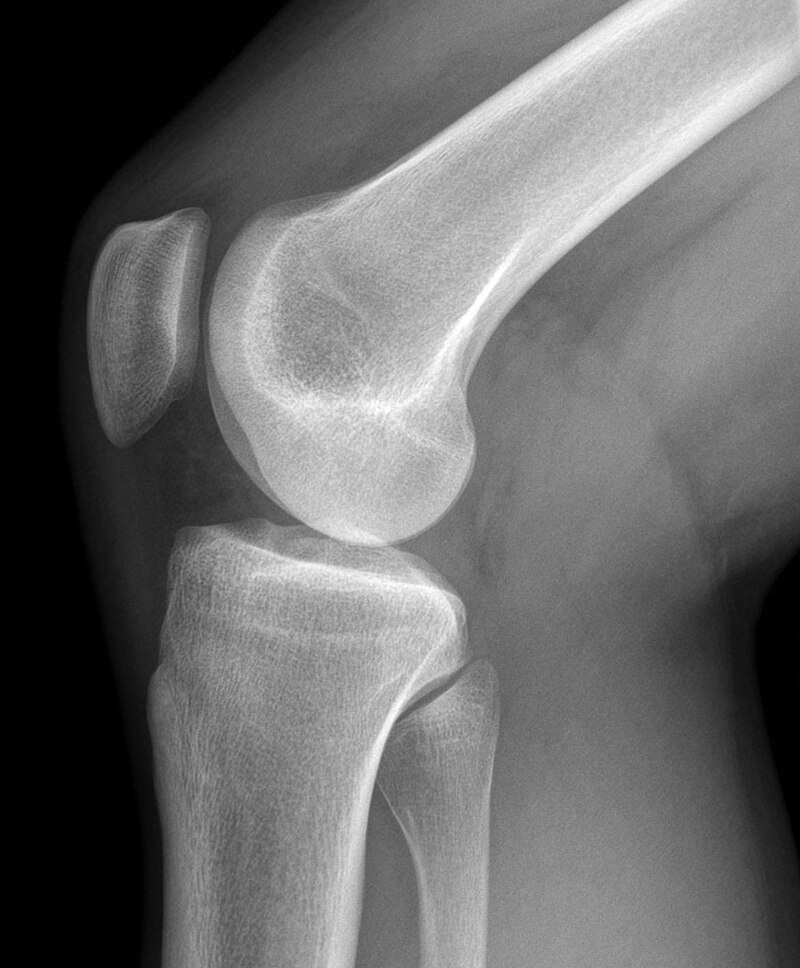
\includegraphics[width=10cm]{Knie-roentgen-r-seite} % https://upload.wikimedia.org/wikipedia/commons/thumb/8/89/Knie-roentgen-r-seite.jpg/800px-Knie-roentgen-r-seite.jpg

\section{Characteristics of X-rays}
\begin{itemize}
\item X-rays are a form of \popup{electromagnetic energy}{Like the
    light.} that occupy a range of frequencies from \popup{30
    petahertz (PHz)}{3x10^16 Hz.} to \popup{30 exahertz
    (EHz)}{3x10^19 Hz}. This places X-rays between ultraviolet light
  and gamma rays on the electromagnetic spectrum
  \cite{bushberg2011essential}.
\item X-rays are a form of \popup{ionizing radiation}{That is capable
    of removing electrons from atoms or molecules, a process known as
    ionization (when an atom or molecule loses or gains electrons, it
    acquires a net electrical charge and becomes an ion).} capable of
  \popup{penetrating soft tissues}{The higher the frequency of the
    X-rays photons, the higher their energy and the higher their
    penetration capability}.
\end{itemize}

\section{Transmission and attenuation}
\begin{itemize}
\item Radiography (X-ray 2D \popup{projection}{Radiography is also a
    projection imaging modality, meaning that each point on the image
    corresponds to information along a straight line through the
    patient}) is a transmission imaging modality where X-rays are
  emitted from a source, pass through the patient, and are detected on
  the other side using a flat (usually digital TFT\footnote{In digital
    X-ray detectors, a TFT array is used to read out electrical
    charges generated by the impact of the X-rays.}) detector.
\item The attenuation properties of different tissues
(e.g., bone, soft tissue, air) modify the homogeneous distribution of
X-rays that enters the patient X-ray, forming the image in the
detector \cite{bushberg2011essential}.
 \cite{bushberg2011essential}.
\end{itemize}
